\section{Efficiency Evaluation \& Simulations}
  \label{section:comparison}
  We offer here a cost and efficiency comparison of this work with
  LVPC~\cite{10.1007/978-3-030-65411-5_18} and Donner~\cite{donner}. We focus on
  these due to their exclusive support of
  virtual channels over any number of base channels. We remind that LVPC
  achieves this via recursion, while Donner
  because it is variadic (c.f.\ Table~\ref{table:comparison-features}).

  We first count the communication, storage and on-chain cost of a virtual
  channel under each protocol. We then simulate the execution of a large number
  of payments among many parties and derive payment latency and fees. We thus
  obtain an end-to-end understanding of both the requirements and the benefits
  each protocol provides.

  \makeatletter%
  \@ifclassloaded{IEEEtran}%
    {\paragraph{Cost calculation}}%
    {\paragraph{Cost calculation.}}%
  \makeatother%
  Consider the setting of $1$
  funder ($P_1$), $1$ fundee ($P_n$) and $n-2$ intermediaries ($P_2, \dots,
  P_{n-1}$) where $P_i$ has a base channel with each of $P_{i-1}$,
  $P_{i+1}$. We compare the off-chain cost of opening
  (Table~\ref{table:comparison:overhead:n-parties:open}) and the on-chain cost
  of unilaterally closing
  (Table~\ref{table:comparison:overhead:n-parties:close}).

  Regarding opening, in
  Table~\ref{table:comparison:overhead:n-parties:open} we measure for each of
  the $3$ protocols the number of communication rounds required, the total
  size of outgoing messages as well as the amount of space for storing
  channel data. We measure from the perspective of the funder, the fundee
  and an intermediary, along with the aggregate for all parties. The
  communication rounds for a party are calculated as its [\#incoming messages +
  \#outgoing messages]/2. The size of outgoing messages and the stored data are
  measured in raw bytes. The data is counted as the sum of the relevant channel
  identifiers ($8$ bytes each, as defined by the Lightning Network
  specification\footnote{\url{https://github.com/lightning/bolts/blob/master/07-routing-gossip.md\#definition-of-short_channel_id}}),
  transaction output identifiers ($36$ bytes), secret keys ($32$ bytes each),
  public keys ($32$ bytes each, compressed form -- these double as party
  identifiers), Schnorr signatures ($64$ bytes each), coins ($8$ bytes each),
  times and timelocks (both $4$ bytes each). UC-specific data is ignored.

  For LVPC, multiple different topologies can support a virtual channel between
  $P_1$ and $P_n$ (all of which need $n-1$ base channels). We here consider the
  case in which the funder $P_1$ first opens one virtual channel with $P_3$ on
  top of channels $(P_1, P_2)$ and $(P_2, P_3)$, then another virtual channel
  with $P_4$ over $(P_1, P_3)$ and $(P_3, P_4)$ and so on up to the $(P_1, P_n)$
  channel, opened over $(P_1, P_{n-1})$ and $(P_{n-1}, P_n)$. We choose this
  topology as $P_1$ cannot assume that there exist any virtual channels between
  other parties (which could be used as shortcuts).

  A subtle byproduct of the above topology is that during the opening phase of
  LVPC every intermediary $P_i$ acts both as a fundee in its virtual channel
  with the funder $P_1$ and as an intermediary in the virtual channel of $P_1$
  with the next party $P_{i+1}$. The above does not apply to the first
  intermediary $P_2$, since it already has a channel with $P_1$ before the
  protocol starts. Table~\ref{table:comparison:overhead:n-parties:open} shows
  the total cost of intermediaries $P_3, \dots, P_{n-1}$. The first intermediary
  $P_2$ incurs instead [intermediary's costs - fundee's costs] for all three
  measured quantities.

  For Elmo, the data are derived assuming a virtual channel opens directly on
  top of $n-1$ base channels. In other words the channel considered is opened
  without the help of recursion and only leverages the variadic property of
  Elmo. In Table~\ref{table:comparison:overhead:n-parties:open} the resources
  calculated for Elmo are exact for $n \geq 4$ parties, whereas for $n = 3$ they
  slightly overestimate.

  For the closing comparison, we measure on-chain transactions' size in
  vbytes\footnote{\url{https://en.bitcoin.it/wiki/Weight_units}}, which map
  directly to on-chain fees and thus are preferable to raw bytes. Using vbytes
  also ensures our comparison remains up-to-date irrespective of the network
  congestion and bitcoin-to-fiat currency exchange rate at the time of reading.
  We use the tool found in
  \url{https://jlopp.github.io/bitcoin-transaction-size-calculator/} to aid size
  calculation. For the case of intermediaries, in order to only show
  the costs incurred due to supporting a virtual channel, we subtract the cost
  the intermediary would pay to close its channel if it was not supporting any
  virtual channel.

  The on-chain number of transactions to close a virtual channel in the case of
  LVPC is calculated as follows: One ``split'' transaction is needed for each
  base channel ($n-1$ in total), plus one ``merge'' transaction per virtual
  channel ($n-2$ in total), plus a single ``refund'' transaction for the virtual
  channel, for a total of $2n-2$ transactions.

  % TODO: understand why number of payments k plays a role in Donner
  % splncs
  %\addtolength{\intextsep}{-30pt}
  \begin{table*}[h!]
    \resizebox{\textwidth}{!}{%
    \begin{tabular}{|l|c|c|c|c|c|c|c|c|c|c|c|}
    \hline
    \multicolumn{12}{|c|}{Open} \\
    \hline
    \multirow{3}{*}{}
              & \multicolumn{3}{|c|}{Funder} & \multicolumn{3}{|c|}{Fundee}
              & \multicolumn{3}{|c|}{Intermediary}
              & \multicolumn{2}{|c|}{Total} \\
    \cline{2-12}
              & \multirow{2}{*}{\shortstack{party \\ rounds}}
              & \multicolumn{2}{|c|}{size} & \multirow{2}{*}{\shortstack{party
              \\ rounds}} & \multicolumn{2}{|c|}{size}
              & \multirow{2}{*}{\shortstack{party \\ rounds}}
              & \multicolumn{2}{|c|}{size} & \multicolumn{2}{|c|}{size} \\
    \cline{3-4} \cline{6-7} \cline{9-12}
              & & sent & stored & & sent & stored & & sent & stored & sent &
              stored \\
    \hline
    LVPC      & $8(n-2)$ & $1381(n-2)$ & $3005(n-2)$ & $7$ & $1254$ & $2936$
              & $16$ & $2989$ & $6385$ & $4370n-8740$ & $9390n-18780$ \\
    \hline
    % my count
    %Donner     & $2$ & $164n + 1934$ & $108n + 2150$ & $1$ & $44n+128$
    %           & $176n+496$ & $1$ & $76n + 2010$ & $132n+2370$
    %           & $132n^2+2390n-2094$ & $76n^2+2066n-1858$ \\
    %\hline
    \multirow{2}{*}{Donner}
              & \multirow{2}{*}{$2$} & \multirow{2}{*}{$184n + 829$}
              & \multirow{2}{*}{\shortstack{$1332.5k+$ \\ $43n+125.5$}}
              & \multirow{2}{*}{$1$} & \multirow{2}{*}{$43n+192.5$}
              & \multirow{2}{*}{\shortstack{$1332.5k+$ \\ $43n+125.5$}}
              & \multirow{2}{*}{$1$} & \multirow{2}{*}{$547$}
              & \multirow{2}{*}{\shortstack{$1332.5k+$ \\ $43n+125.5$}}
              & \multirow{2}{*}{$774n-71$}
              & \multirow{2}{*}{\shortstack{$1332.5kn +$ \\ $43n^2 + 125.5n$}}
              \\
              & & & & & & & & & & & \\
              % For Donner, I drew the storage numbers from
              % https://eprint.iacr.org/2021/855.pdf, p. 22. I'm not sure what
              % pid is, so these numbers may have to be revised.
    \hline
    \multirow{3}{*}{Elmo}
              & \multirow{3}{*}{$6$} &
              \multirow{3}{*}{\shortstack{$32n^3-128n^2$ \\
              $+544n-276$}} &
              \multirow{3}{*}{\shortstack{$\frac{128}{3}n^3-128n^2$ \\
              $+\frac{1276}{3}n+220$}} &
              \multirow{3}{*}{$6$}
              & \multirow{3}{*}{\shortstack{$32n^3-128n^2$ \\
              $+544n-340$}} &
              \multirow{3}{*}{\shortstack{$\frac{128}{3}n^3-128n^2$ \\
              $+\frac{1276}{3}n+220$}} &
              \multirow{3}{*}{$12$}
              & \multirow{3}{*}{\shortstack{$96n^3-256n^2$ \\
              $+404n-40$}}
              & \multirow{3}{*}{\shortstack{$96n^3-256n^2$ \\
              $+468n+88$}}
              & \multirow{3}{*}{\shortstack{$96n^4-384n^3+$ \\
              $724n^2+240n-792$}} &
              \multirow{3}{*}{\shortstack{$96n^4-\frac{1088}{3}n^3+$ \\
              $660n^2+\frac{8}{3}n+520$}}\\
              & & & & & & & & & & & \\
              & & & & & & & & & & & \\
    \hline
    \end{tabular}}
    \caption{Open efficiency comparison of virtual channel protocols with $n$
    parties and $k$ payments}
    \label{table:comparison:overhead:n-parties:open}
  \end{table*}
  % splncs
  %\addtolength{\intextsep}{30pt}

  Regarding closing, in Table~\ref{table:comparison:overhead:n-parties:close} we
  measure for each of the three protocols the worst-case on-chain cost a party
  would need to incur in order to unilaterally close its channel. The cost is
  measured both in the number of transactions and in their total size.

  For the two endpoints (funder and fundee), the cost of unilaterally closing
  the virtual channel is reported. On the other hand, for each intermediary we
  report the cost of closing a base channel. We also present the worst-case
  total on-chain cost,
  aggregated over all parties. Note that the latter cost is not simply the sum
  of the worst-case costs of all parties, as one party's worst case is not
  necessarily the worst case of another. This cost rather represents the maximum
  possible load an instantiation of each protocol could add to the blockchain
  when closing.

  % splncs
  %\addtolength{\intextsep}{-30pt}
  \begin{table*}[h!]
    \begin{minipage}{\textwidth}
    \centering
    \begin{tabular}{|l|c|c|c|c|c|c|c|c|}
    \hline
    \multicolumn{9}{|c|}{Unilateral Close} \\
    \hline
              & \multicolumn{2}{|c|}{Intermediary}
              & \multicolumn{2}{|c|}{Funder} & \multicolumn{2}{|c|}{Fundee}
              & \multicolumn{2}{|c|}{Total} \\
    \hline
              & \#txs & size & \#txs & size & \#txs & size & \#txs & size \\
    \hline
    LVPC      & $3$ & $627$ & $2$ & $383$ & $2$ & $359$ & $2n-2$ & $435n -
              510.5$ \\
    \hline
    Donner    & $1$ & $204.5$ & $4$ & $704 + 43n$ & $1$ & $136.5$ & $2n$ & $458n
              - 26$ \\
    \hline
    Elmo      & $1$ & $297.5$ & $3$ & $376$ & $3$ & $376$
              & $n+1$ & $254.5n-133$ \\
    \hline
    \end{tabular}
    \end{minipage}
    \caption{On-chain worst-case closing efficiency comparison of virtual
    channel protocols with $n$ parties}
    \label{table:comparison:overhead:n-parties:close}
  \end{table*}
  % splncs
  %\addtolength{\intextsep}{30pt}

  We note that Elmo exploits
  MuSig2~\cite{DBLP:journals/dcc/MaxwellPSW19,DBLP:conf/crypto/NickRS21} to
  reduce both its
  on-chain and storage footprint: the $n$ signatures that are needed to spend
  each virtual and bridge output can be securely reduced to a single aggregate
  signature. The same cannot be said for
  Donner, since this technique cannot optimise away the $n$ outputs of the
  funder's transaction $\tx^{\mathtt{vc}}$. Likewise LVPC cannot gain a linear
  improvement with this optimisation, since each of its relevant transactions
  (``split'', ``merge'' and ``refund'') needs constant signatures.

  \makeatletter%
  \@ifclassloaded{IEEEtran}%
    {\paragraph{Payment simulations}}%
    {\paragraph{Payment simulations.}}%
  \makeatother%
  We implemented a simulation
  framework\footnote{\url{gitlab.com/anonymised-submission-8778e084/virtual-channels-simulation}}
  in which a list of randomly generated payments are carried out.
  A single simulation is parametrised by a list of payments
  (sender, receiver, value triples), the protocol (Elmo, Donner, LVPC, LN or
  on-chain only), which future payments each payer knows and the utility
  function it maximises. The knowledge function defines which future payments
  inform each decision. Several knowledge functions are provided, such as full
  knowledge of all future payments and knowledge of the payer's next $m$
  payments. All simulations presented here were carried out with
  each party knowing its next $m=10$ payments, as we decided
  this is a realistic knowledge function.

  The utility of a payment is high when its latency and fees are
  low, it increases the payer's network centrality, and reduces
  distance from other parties. We give more weight to low latency
  and fees, then to small distance and lastly to high centrality.
  Each payment is carried out by dry-running all known future
  payments with the three possible payment kinds (simply
  on-chain, opening a new channel, using existing
  channels), comparing their utility and executing the best one.
  Recognising the arbitrary nature of the concrete weights, we
  chose them before running our simulations in order to minimise
  bias.

  The simulation outputs extensive data on the progress of each run. Our
  simulation framework is of independent interest, as it is built to be flexible
  and reusable for a variety of payment network protocol evaluations. We here
  show the performance of the $3$ protocols with respect to the metrics payment
  channels aim to improve, namely payment latency and fees.

  Due to the privacy guarantees of LN, we are unable to obtain real-world
  off-chain payment data. We therefore generate payments randomly. More
  specifically, we provide three different payment topologies to mimic
  different usage schemes: First, each party has a preferred receiver, chosen
  uniformly at the beginning, which it pays half the time, the other half
  choosing the payee uniformly at random. Each payment value is chosen
  uniformly at random from the $[0, \max]$ range, for $\max =
  \frac{(\text{initial coins}) \cdot \text{\#players}}{\text{\#payments}}$. We
  employ $1000$ parties. This scenario occurs when new users are onboarded with
  the intent to primarily pay a single counterparty, but sporadically pay
  others as well. Second, in an attempt to emulate real-world payment
  distributions, the value and number of incoming payments of each player are
  drawn from the zipf~\cite{powers-1998-applications} distibution with
  parameter $2$. Each payment value is chosen according to the
  zipf(2.16) distribution, moved to have a mean equal to $\frac{\max}{2}$. We
  consider $500$ parties. Third, all choices are made uniformly at random, with
  each payment chosen uniformly from $[0, \max]$, employing a total of $3000$
  parties. For all scenarios the payer of each payment is chosen uniformly at
  random, no channels exist initially, and all parties initially own the same
  number of coins on-chain. The
  number of parties is chosen to ensure the simulation completes within a
  reasonable length of time.

  In order to avoid bias, we simulate each
  protocol with the same payments. We simulate each scenario with $20$
  distinct sets of payments and keep the average. Figs.~\ref{graph:delays}
  and~\ref{graph:fees} show the per-payment latency and fee
  respectively. Scale does not begin at zero for better visibility. Average
  latency is high as it describes the whole run, including slow on-chain
  payments and channel openings. Total fees are calculated by summing the fee
  of each ``basic'' event (e.g., paying an intermediary for its service). None
  of the $3$ protocols provide fee recommendations, so we use the same baseline
  fees for the same events in all $3$ to avoid bias. These
  fees are not systematically chosen, therefore Fig.~\ref{graph:fees} provides
  relative, not absolute, fees. As can be seen, Elmo is the best or on par with
  the best protocol in every case.

  \addtolength{\intextsep}{-15pt}
  \begin{figure*}
  \begin{subfigure}{.3293\textwidth}
  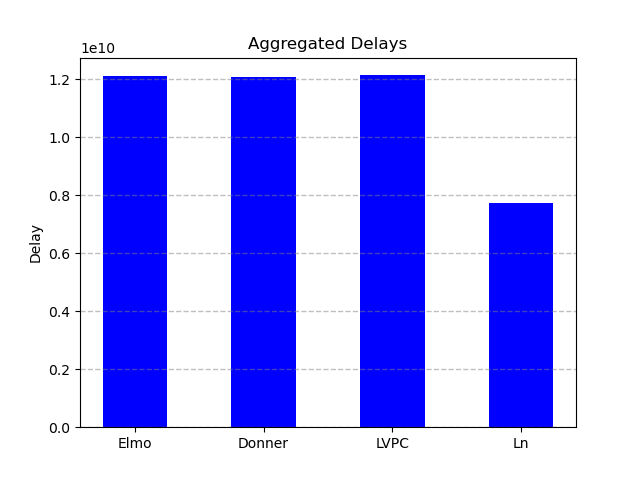
\includegraphics[width=\textwidth]{../simulation/Delays_power_law.png}
  \end{subfigure}
  \begin{subfigure}{.3293\textwidth}
  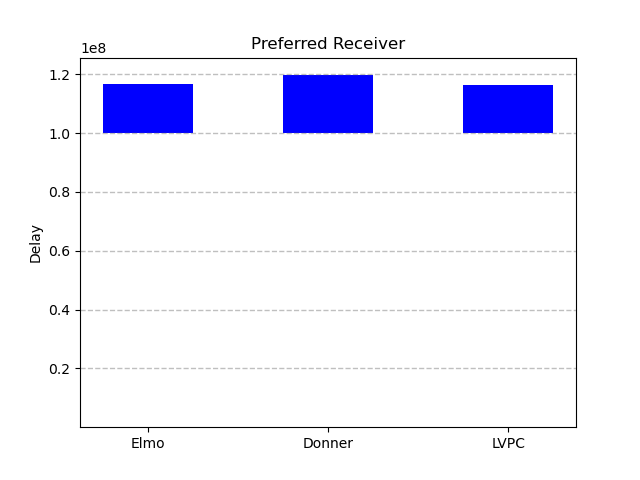
\includegraphics[width=\textwidth]{../simulation/Delays_preferred_receiver.png}
  \end{subfigure}
  \begin{subfigure}{.3293\textwidth}
  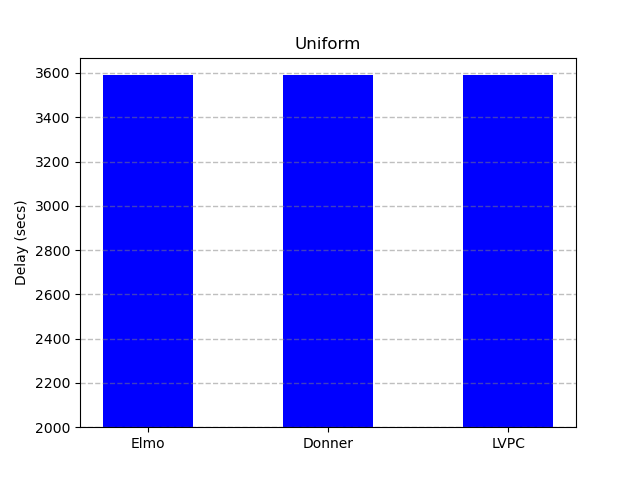
\includegraphics[width=\textwidth]{../simulation/Delays_uniform.png}
  \end{subfigure}
  \caption{Average per-payment delay (including both on- and off-chain) in
  seconds. Less is better.}
  \label{graph:delays}
  \end{figure*}
  \begin{figure*}
  \begin{subfigure}{.3293\textwidth}
  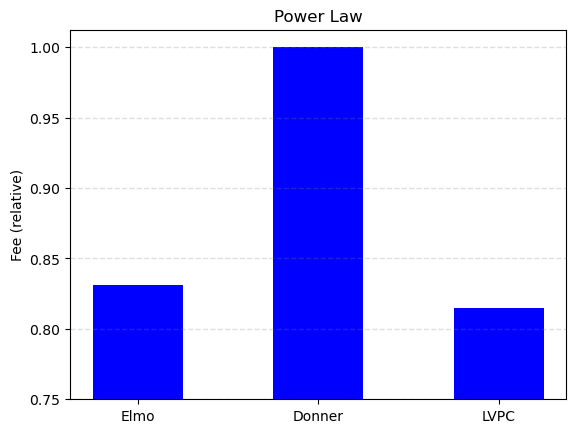
\includegraphics[width=\textwidth]{../simulation/Fees_power_law.png}
  \end{subfigure}
  \begin{subfigure}{.3293\textwidth}
  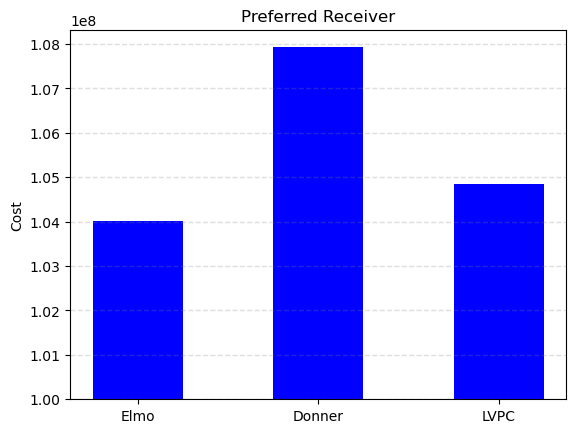
\includegraphics[width=\textwidth]{../simulation/Fees_preferred_receiver.png}
  \end{subfigure}
  \begin{subfigure}{.3293\textwidth}
  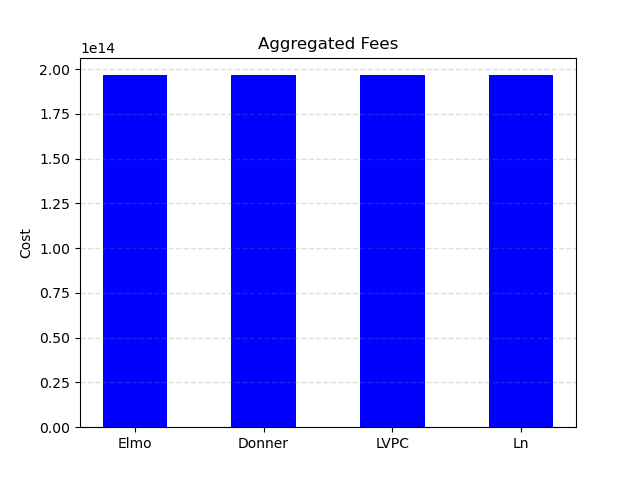
\includegraphics[width=\textwidth]{../simulation/Fees_uniform.png}
  \end{subfigure}
  \caption{Average per-payment relative fee. Less is better.}
  \label{graph:fees}
  \end{figure*}
  \addtolength{\intextsep}{15pt}
